%\documentclass{beamer}
\documentclass[9pt, table]{beamer}

\usepackage[slovene]{babel}
\usepackage{amsfonts,amssymb}
\usepackage[utf8]{inputenc}
%\usepackage{lmodern}
\usepackage[T1]{fontenc}

\usepackage{mathptmx}
\usepackage{helvet}
\usepackage{courier}

\setbeamercovered{transparent}

\usetheme{Warsaw}
\usecolortheme{rose}

\newtheorem{izrek}{Izrek}
\newtheorem{definicija}{Definicija}
\newtheorem{primer}{Primer}
\newtheorem{trditev}{Trditev}
\newtheorem{lema}{Lema}
\newtheorem{oznaka}{Oznaka}

\newcommand{\R}{\mathbb R}
\newcommand{\N}{\mathbb N}
\newcommand{\Z}{\mathbb Z}
\newcommand{\C}{\mathbb C}
\newcommand{\Q}{\mathbb Q}

\newcommand{\pojem}[1]{\textsc{#1}}


\title{Minimalne ploskve}
\author{Tjaša Vrhovnik}

\institute{Mentor: akad.~prof.~dr.~Franc Forstnerič\\
	Univerza v Ljubljani\\
	Fakulteta za matematiko in fiziko\\
	Matematika -- 2.~stopnja}
\date{januar 2022}

\begin{document}

%%%%%%%%%%%%%%%%%%%%%%%%%%%%%%%%%%%%%%%%%%%

\begin{frame}
\titlepage
\end{frame}

%%%%%%%%%%%%%%%%%%%%%%%%%%%%%%%%%%%%%%%%%%%

\begin{frame}
\frametitle{Struktura magistrskega dela}

\begin{enumerate}
\item Uvod
\item Osnovni pojmi
\item Minimalne ploskve
\item Izreki o aproksimaciji in interpolaciji minimalnih ploskev
\end{enumerate}

\end{frame}

%%%%%%%%%%%%%%%%%%%%%%%%%%%%%%%%%%%%%%%%%%%

\begin{frame}
\frametitle{Kratka zgodovina}

\begin{itemize}
\item {\color{blue} L.~Euler} opiše katenoido (l.~1744)
\item {\color{blue} J.~L.~Lagrange} enačba za minimalne grafe (l.~1762)
\item {\color{blue} J.~B.~Meusnier} ploskve z ničelno povprečno ukrivljenostjo lokalno minimizirajo površino
\item {\color{blue} J.~Plateau} poskusi z milnico
\item Razvoj kompleksne analize in diferencialne geometrije -- reprezentacijska formula (l.~1866)
\item {\color{blue} T.~Rad\'o} (l.~1930) in {\color{blue} J.~Douglas} (l.~1931) rešita Plateaujev problem 
\end{itemize}

\end{frame}

%%%%%%%%%%%%%%%%%%%%%%%%%%%%%%%%%%%%%%%%%%%

\begin{frame}
\frametitle{Osnovni pojmi}

\begin{definicija}
{\color{blue} Riemannova ploskev} je kompleksna mnogoterost kompleksne dimenzije $1$.
\end{definicija}

\begin{definicija}
Gladka preslikava $f \colon M \to N$ med gladkima mnogoterostma se imenuje 
{\color{blue} imerzija} v točki $p \in M$, če je njen diferencial $df_{p} \colon T_{p}M \to T_{f(p)}N$ injektiven.
\end{definicija}

Konformne imerzije razreda $\mathcal{C}^2$ iz odprte Riemannove ploskve v Evklidski prostor 
\begin{gather*}
x \colon M \to \mathbb{R}^{n}, \ n \geq 3.
\end{gather*}

\end{frame}

%%%%%%%%%%%%%%%%%%%%%%%%%%%%%%%%%%%%%%%%%%%

\begin{frame}
\frametitle{Osnovni pojmi}

\begin{definicija}
{\color{blue} Povprečna ukrivljenost} ploskve $S$ v točki $p$ in normalni smeri $N$ je povprečje glavnih ukrivljenosti,
\begin{equation}
H^{N}(p) = \frac{1}{2} \left(\kappa _{1}^{N}(p) + \kappa _{2}^{N}(p) \right).
\end{equation}

{\color{blue} Vektor povprečne ukrivljenosti} v točki $p$ je vektor $\textbf{\textup{H}}$, ki zadošča $H^{N}(p) = \textbf{\textup{H}} \cdot N$ za vsak $N \in N_{p}S$.
\end{definicija}

\end{frame}

%%%%%%%%%%%%%%%%%%%%%%%%%%%%%%%%%%%%%%%%%%%

\begin{frame}
\frametitle{Osnovni pojmi}

\begin{definicija}
Naj bo $x \colon M \to \R^{n}$ harmonična preslikava. Njen {\color{blue} pretok} je homomorfizem grup $\mathrm{Flux}_{x} \colon H_{1} (M, \Z) \to \R^{n}$, definiran s predpisom 
\begin{equation} 
\mathrm{Flux}_{x} ([C]) = \int_{C} {d^{c} x}.
\end{equation}
\end{definicija}
\pause

\begin{definicija}
Naj bo $K$ kompaktna podmnožica Riemannove ploskve $M$. Njena {\color{blue} holomorfna ogrinjača} je množica 
\begin{equation}
\widehat{K}_{\mathcal{O}(M)} = \{p \in M ; \ |f(p)| \leq \max_{K} |f| \ \text{za vse} \ f \in \mathcal{O}(M) \}.
\end{equation}
Če velja $K = \widehat{K}_{\mathcal{O}(M)}$, potem $K$ imenujemo {\color{blue} Rungejeva množica}.
\end{definicija}

\end{frame}

%%%%%%%%%%%%%%%%%%%%%%%%%%%%%%%%%%%%%%%%%%%

\begin{frame}
\frametitle{Minimalne ploskve}

\begin{definicija}
Naj bo $M$ gladka kompaktna ploskev z robom, $n \geq 3$ in naj bo preslikava $x \colon M \to \R^{n}$ imerzija razreda $\mathcal{C}^2$. {\color{blue} Variacija preslikave x s fiksnim robom} je 1-parametrična družina $\mathcal{C}^2$ preslikav 
\begin{gather}
x^{t} \colon M \to \R^{n}, \quad t \in (-\varepsilon, \varepsilon) \subset \R,
\end{gather}
če je $x^0 = x$ in za vse $t$ z intervala velja $x^{t} = x$ na $bM$.
\end{definicija}
\pause

\begin{definicija} [Minimalna ploskev]
Naj bo $x \colon M \to \R^{n}$ imerzija razreda $\mathcal{C}^2$. Sliko $x(M)$ imenujemo {\color{blue} minimalna ploskev}, če za vsako kompaktno domeno $D \subset M$ z gladkim robom $bD$ in vsako gladko variacijo $x^{t}$ preslikave $x$ s fiksnim robom velja
\begin{equation} 
\frac{d}{dt} \Big|_{t=0} \mathrm{Area} \left(x^{t}(D)\right) = 0.
\end{equation}
Ekvivalentno pravimo, da je minimalna ploskev stacionarna točka ploskovnega funkcionala $\mathrm{Area}$.
\end{definicija}

\end{frame}

%%%%%%%%%%%%%%%%%%%%%%%%%%%%%%%%%%%%%%%%%%%

\begin{frame}
\frametitle{Minimalne ploskve}

\begin{izrek}
Naj bo $M$ odprta Riemannova ploskev, $n \geq 3$ in $x = (x_1, \dots , x_n) \colon M \to \R^{n}$ konformna imerzija razreda $\mathcal{C}^2$. Naslednje trditve so ekvivalentne.
\begin{enumerate}
	\item $x$ je minimalna ploskev\index{minimalna ploskev}.
	\item Vektorsko polje povprečne ukrivljenosti preslikave $x$ je ničelno, tj.~$\textbf{\textup{H}} = 0$.
	\item $x$ je harmonična.
	\item 1-forma $ \partial{x} = (\partial{x_1}, \dots , \partial{x_n})$ z vrednostmi v $\C^{n}$ je holomorfna in velja
			\begin{equation} \label{eq:partialx^2 = 0}
			(\partial{x_1})^2 + \cdots + (\partial{x_n})^2 = 0.
			\end{equation}
	\item Naj bo $\theta$ holomorfna 1-forma na $M$, ki ni nikjer enaka $0$. Potem je preslikava $f = 2\partial{x} / \theta \colon M \to \C^{n}$ holomorfna z 				vrednostmi v punktirani ničelni kvadriki
			\begin{equation}	
			\textbf{\textup{A}}_{*} = \{ (z_1, \dots , z_n) \in \C^{n}_{*} ; \ z_{1}^{2} + \cdots + z_{n}^{2} = 0 \}.
			\end{equation}	
\end{enumerate}
Nadalje je Riemannova metrika na $M$, inducirana s konformno imerzijo $x$, enaka
	\begin{equation} \label{eq:|dx|^2=2|partialx|^2}
	g = x^{*} ds^2 = |dx_1|^2 + \cdots + |dx_n|^2 = 2 (|\partial{x_1}|^2 + \cdots |\partial{x_n}|^2).
	\end{equation}			
\end{izrek}

\end{frame}

%%%%%%%%%%%%%%%%%%%%%%%%%%%%%%%%%%%%%%%%%%%

\begin{frame}
\frametitle{Minimalne ploskve}

\begin{izrek}[Enneper-Weierstrassova formula]
Naj bo $n \geq 3$ in $M$ odprta Riemannova ploskev. Na njej izberimo holomorfno 1-formo $\phi = (\phi_{1}, \dots , \phi_{n})$ z vrednostmi v $\C^{n}$, ki je povsod neničelna in zadošča 
\begin{enumerate}
\item $ \sum_{j=1}^{n} \phi_{j}^{2} = 0$,
\item $ \Re \int_{C} \phi = 0 $ za vse $[C] \in H_{1} (M, \Z)$.
\end{enumerate}
Potem za poljuben izbor točk $p_0 \in M$ in $x_0 \in \R^{n}$ predpis $x \colon M \to \R^{n}$,
\begin{align}
x(p) = x_0 + \Re \int_{p_0}^{p} \phi, \quad p \in M,
\end{align}
podaja dobro definirano konformno minimalno imerzijo. Zanjo velja
\begin{align}
2 \partial{x} = \phi \quad \text{in} \quad g = x^{*} ds^2 = |dx|^2 = \frac{1}{2} |\phi|^2.
\end{align}
\end{izrek}

\end{frame}

%%%%%%%%%%%%%%%%%%%%%%%%%%%%%%%%%%%%%%%%%%%

\begin{frame}
\frametitle{Minimalne ploskve in holomorfne ničelne krivulje}

\begin{definicija}
Naj bo $M$ odprta Riemannova ploskev in $n \geq 3$. Holomorfno imerzijo $z = (z_{1}, \dots , z_{n}) \colon M \to \C^{n}$, za katero velja
$(\partial{z_{1}})^2 + \cdots + (\partial{z_{n}})^2 = 0$, imenujemo {\color{blue} holomorfna ničelna krivulja}\index{holomorfna ničelna krivulja} v $\C^{n}$.
\end{definicija}
\pause

Če v Enneper-Weierstrassovi formuli velja še
$ \int_{C} \phi = 0 \ \text{za vse} \ [C] \in H_{1} (M, \Z) $,
potem za poljuben izbor točk $p_0 \in M$ in $z_0 \in \C^{n}$ predpis $z \colon M \to \C^{n}$,
\begin{align}
z(p) = z_0 + \int_{p_0}^{p} \phi, \quad p \in M,
\end{align}
podaja dobro definirano holomorfno ničelno krivuljo. Zanjo velja
\begin{align}
\partial{z} = \phi \quad \text{in} \quad z^{*} ds^2 = |dz|^2 = |\partial{z}|^2 = |\phi|^2.
\end{align}

\end{frame}

%%%%%%%%%%%%%%%%%%%%%%%%%%%%%%%%%%%%%%%%%%%

\begin{frame}
\frametitle{Aproksimacija in interpolacija minimalnih ploskev}

Cilj: dokazati aproksimacijski in interpolacijski izrek tipa Mergelyana in Weierstrassa za konformne minimalne ploskve in holomorfne ničelne krivulje

\begin{itemize}
\item klasični izreki za holomorfne funkcije
\item Morsejeva teorija
\item konstrukcija poti s predpisanimi integrali (Gromov)
\end{itemize}
\vspace{0.4cm}
\pause

Načrt: 
\begin{itemize}
\item aproksimacija in interpolacija preslikav v punktirano ničelno kvadriko
\item nekritičen primer
\item splošen primer
\end{itemize}

\end{frame}

%%%%%%%%%%%%%%%%%%%%%%%%%%%%%%%%%%%%%%%%%%%

\begin{frame}
\frametitle{Aproksimacija in interpolacija minimalnih ploskev}

\begin{definicija}
Naj bo $M$ gladka ploskev. Kompaktno podmnožico v $M$ oblike $S = K \cup E$ imenujemo {\color{blue} dopustna množica}, kjer je $K$ končna unija paroma disjunktnih kompaktnih domen s kosoma zvezno odvedljivimi robovi v $M$ ter $E = S \setminus K^\circ$ unija končno mnogo paroma disjunktnih gladkih Jordanovih lokov in zaprtih Jordanovih krivulj, ki se dotikajo $K$ kvečjemu v svojih krajiščih in sekajo rob $K$ transverzalno.
\end{definicija}
\pause

\begin{definicija}
Naj bo $S = K \cup E$ dopustna podmnožica Riemannove ploskve $M$ in $\theta$ povsod neničelna holomorfna 1-forma, definirana v okolici $S \subset M$.
Naj bosta $n \geq 3$ in $r \in \N$. {\color{blue} Posplošena konformna minimalna imerzija} $S \to \R^{n}$ razreda $\mathcal{C}^{r}$ je par $(x, f \theta)$, kjer je $x \colon S \to \R^{n}$ preslikava razreda  $\mathcal{C}^{r}$, njena zožitev na $S^\circ = K^\circ$ je konformna minimalna imerzija in preslikava $f \in \mathcal{A}^{r-1}(S, \textbf{\textup{A}}_{*})$ zadošča naslednjima pogojema:
\begin{enumerate}
\item na množici $K$ velja $f \theta = 2 \partial x$;
\item za vsako gladko pot $\alpha$ v $M$, ki parametrizira povezano komponento množice $E = \overline{S \setminus K}$, velja $ \Re(\alpha^{*}(f \theta)) = \alpha^{*}(dx) = d(x \circ \alpha)$.
\end{enumerate}
\end{definicija}

\end{frame}

%%%%%%%%%%%%%%%%%%%%%%%%%%%%%%%%%%%%%%%%%%%

\begin{frame}
\frametitle{Aproksimacija in interpolacija minimalnih ploskev}

\begin{trditev} [Nekritičen primer glavnega izreka]
Naj bo $M$ odprta Riemannova ploskev in $\theta$ povsod neničelna holomorfna 1-forma na $M$.
Predpostavimo, da je $S$ taka povezana dopustna množica v $M$, da inkluzija $S \hookrightarrow M$ porodi izomorfizem $H_{1}(S,\Z) \stackrel{\cong}{\longrightarrow} H_{1}(M,\Z)$ prvih homoloških grup. Naj bo $A=\{a_{1}, \dots , a_{k} \} \subset S$ končna množica točk in $r, s \in \N$. Tedaj velja naslednje:
\begin{enumerate}
\item 
Vsako posplošeno konformno minimalno imerzijo $(x, f\theta) \in \textup{GCMI}^{r}(S,\R^{n})$ lahko v $\mathcal{C}^{r}(S)$ aproksimiramo s polnimi konformnimi minimalnimi imerzijami $X \colon M \to \R^{n}$, za katere je $\mathrm{Flux}_{X} = \mathrm{Flux}_{x}$. 
\item
Vsako posplošeno ničelno krivuljo $(z, f\theta) \in \textup{GNC}^{r}(S,\C^{n})$ lahko v $\mathcal{C}^{r}(S)$ aproksimiramo s polnimi holomorfnimi ničelnimi krivuljami $Z \colon M \to \C^{n}$.
\end{enumerate}
Dodatno, preslikave $X$ oz.~$Z$ lahko izberemo tako, da se s preslikavama $x$ oz.~$z$ ujemajo v točkah množice $A$ ter do danega končnega reda v točkah množice $A \cap S^{\circ}$.
\end{trditev}

\end{frame}

%%%%%%%%%%%%%%%%%%%%%%%%%%%%%%%%%%%%%%%%%%%

\begin{frame}
\frametitle{Aproksimacija in interpolacija minimalnih ploskev}

\begin{izrek}
Naj bo $M$ odprta Riemannova ploskev, $\theta$ povsod neničelna holomorfna 1-forma na $M$, $n \geq 3$ in $r \geq 1$.
Naj bo $S$ dopustna Rungejeva množica v $M$ in $\Lambda \subset M$ zaprta diskretna podmnožica. 
Naj bo $x \colon S \to \R^{n}$ posplošena konformna minimalna imerzija razreda $\mathcal{C}^{r}(S, \R^{n})$, ki je konformna minimalna imerzija v okolici vsake točke iz $\Lambda$.

Za izbrane $\varepsilon > 0$, preslikavo $k \colon \Lambda \to \N$ in homomorfizem grup $\mathfrak{p} \colon H_{1}(M,\Z) \to \R^{n}$, \ $\mathfrak{p}|_{H_{1}(S,\Z)} = \mathrm{Flux}_{x}$ obstaja konformna minimalna imerzija $\tilde{x} \colon M \to \R^{n}$, za katero velja:
\begin{enumerate}
\item $||\tilde{x} - x||_{\mathcal{C}^{r}(S)} < \varepsilon$;
\item razlika $\tilde{x}-x$ je ničelna do reda $k(p)$ v vsaki točki $p\in \Lambda$;
\item $\mathrm{Flux}_{\tilde{x}} = \mathfrak{p}$ na $H_{1}(M,\Z)$;
\item če je $n\geq5$ in je $x \colon \Lambda \to \R^{n}$ injektivna preslikava, potem je $\tilde{x}$ injektivna imerzija;
\item če je $n=4$ in ima $x$ enostavne dvojne točke na množici $\Lambda$, potem je $\tilde{x}$ imerzija z enostavnimi dvojnimi točkami na $\Lambda$.
\end{enumerate}
\end{izrek}

\end{frame}

%%%%%%%%%%%%%%%%%%%%%%%%%%%%%%%%%%%%%%%%%%%

\begin{frame}
\frametitle{Aproksimacija in interpolacija minimalnih ploskev}

\begin{izrek} [Mittag-Lefflerjev izrek za konformne minimalne imerzije]
Naj bo $M$ odprta Riemannova ploskev, $A \subset M$ njena zaprta diskretna podmnožica, $U \subset M$ okolica množice $A$, ki je Rungejeva v $M$, in $n \geq 3$.
Predpostavimo, da je $x \colon U \setminus A \to \R^{n}$ konformna minimalna imerzija, pripadajočo 1-formo $\partial x$ pa lahko meromorfno razširimo na $U$ s poli v točkah množice $A$.
Tedaj obstaja taka polna konformna minimalna imerzija $\tilde{x} \colon M \setminus A \to \R^{n}$, da je razlika $\tilde{x}-x$ harmonična na množici $A$.
Natančneje, 1-formo $\partial \tilde{x}$ lahko meromorfno razširimo na $M$ s poli v točkah množice $A$.
\end{izrek}

\end{frame}

%%%%%%%%%%%%%%%%%%%%%%%%%%%%%%%%%%%%%%%%%%%

\begin{frame}
\frametitle{Primeri minimalnih ploskev -- katenoida}

\begin{align*}
x &\colon \R^{2} \to \R^{3} \\
x(u,v) &= (\cos u \cdot \cosh v, \sin u \cdot \cosh v, v)
\end{align*}
%
\begin{center}
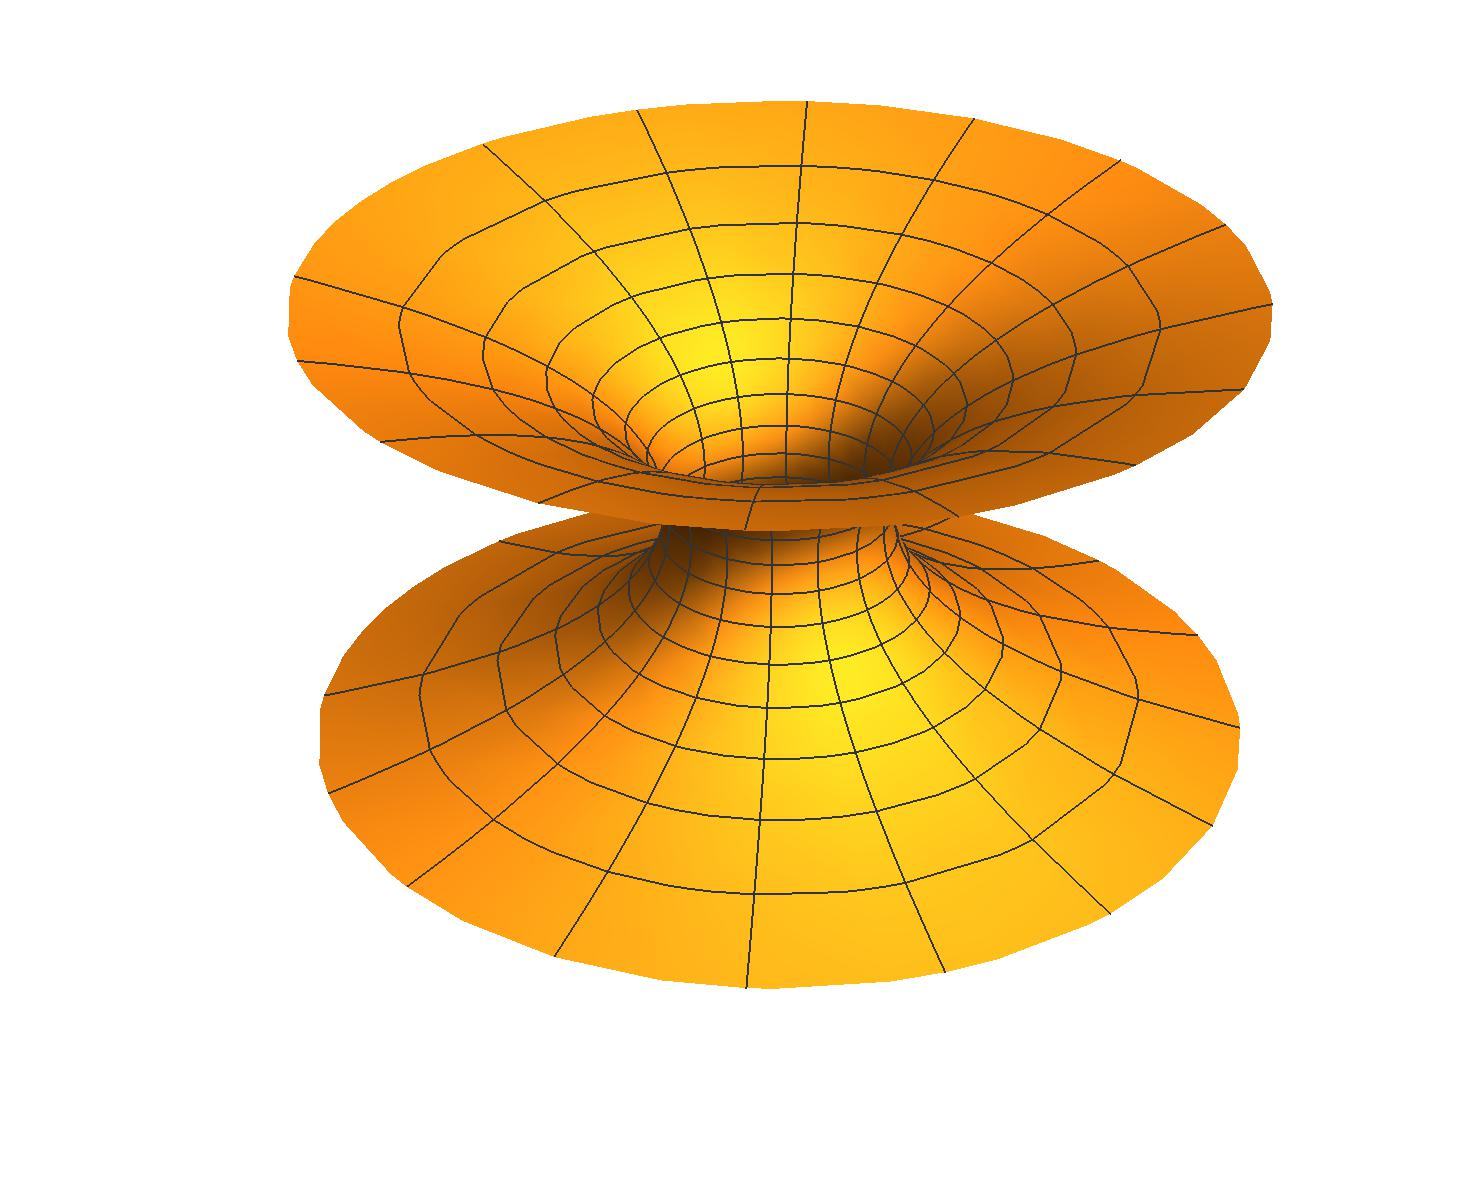
\includegraphics[scale=0.5]{katenoida.jpg}
\end{center}

\end{frame}

%%%%%%%%%%%%%%%%%%%%%%%%%%%%%%%%%%%%%%%%%%%

\begin{frame}
\frametitle{Primeri minimalnih ploskev -- helikoid}

\begin{align*}
x &\colon \R^{2} \to \R^{3} \\
x(u,v) &= (\sin u \cdot \sinh v, -\cos u \cdot \sinh v, u)
\end{align*}
%
\begin{center}
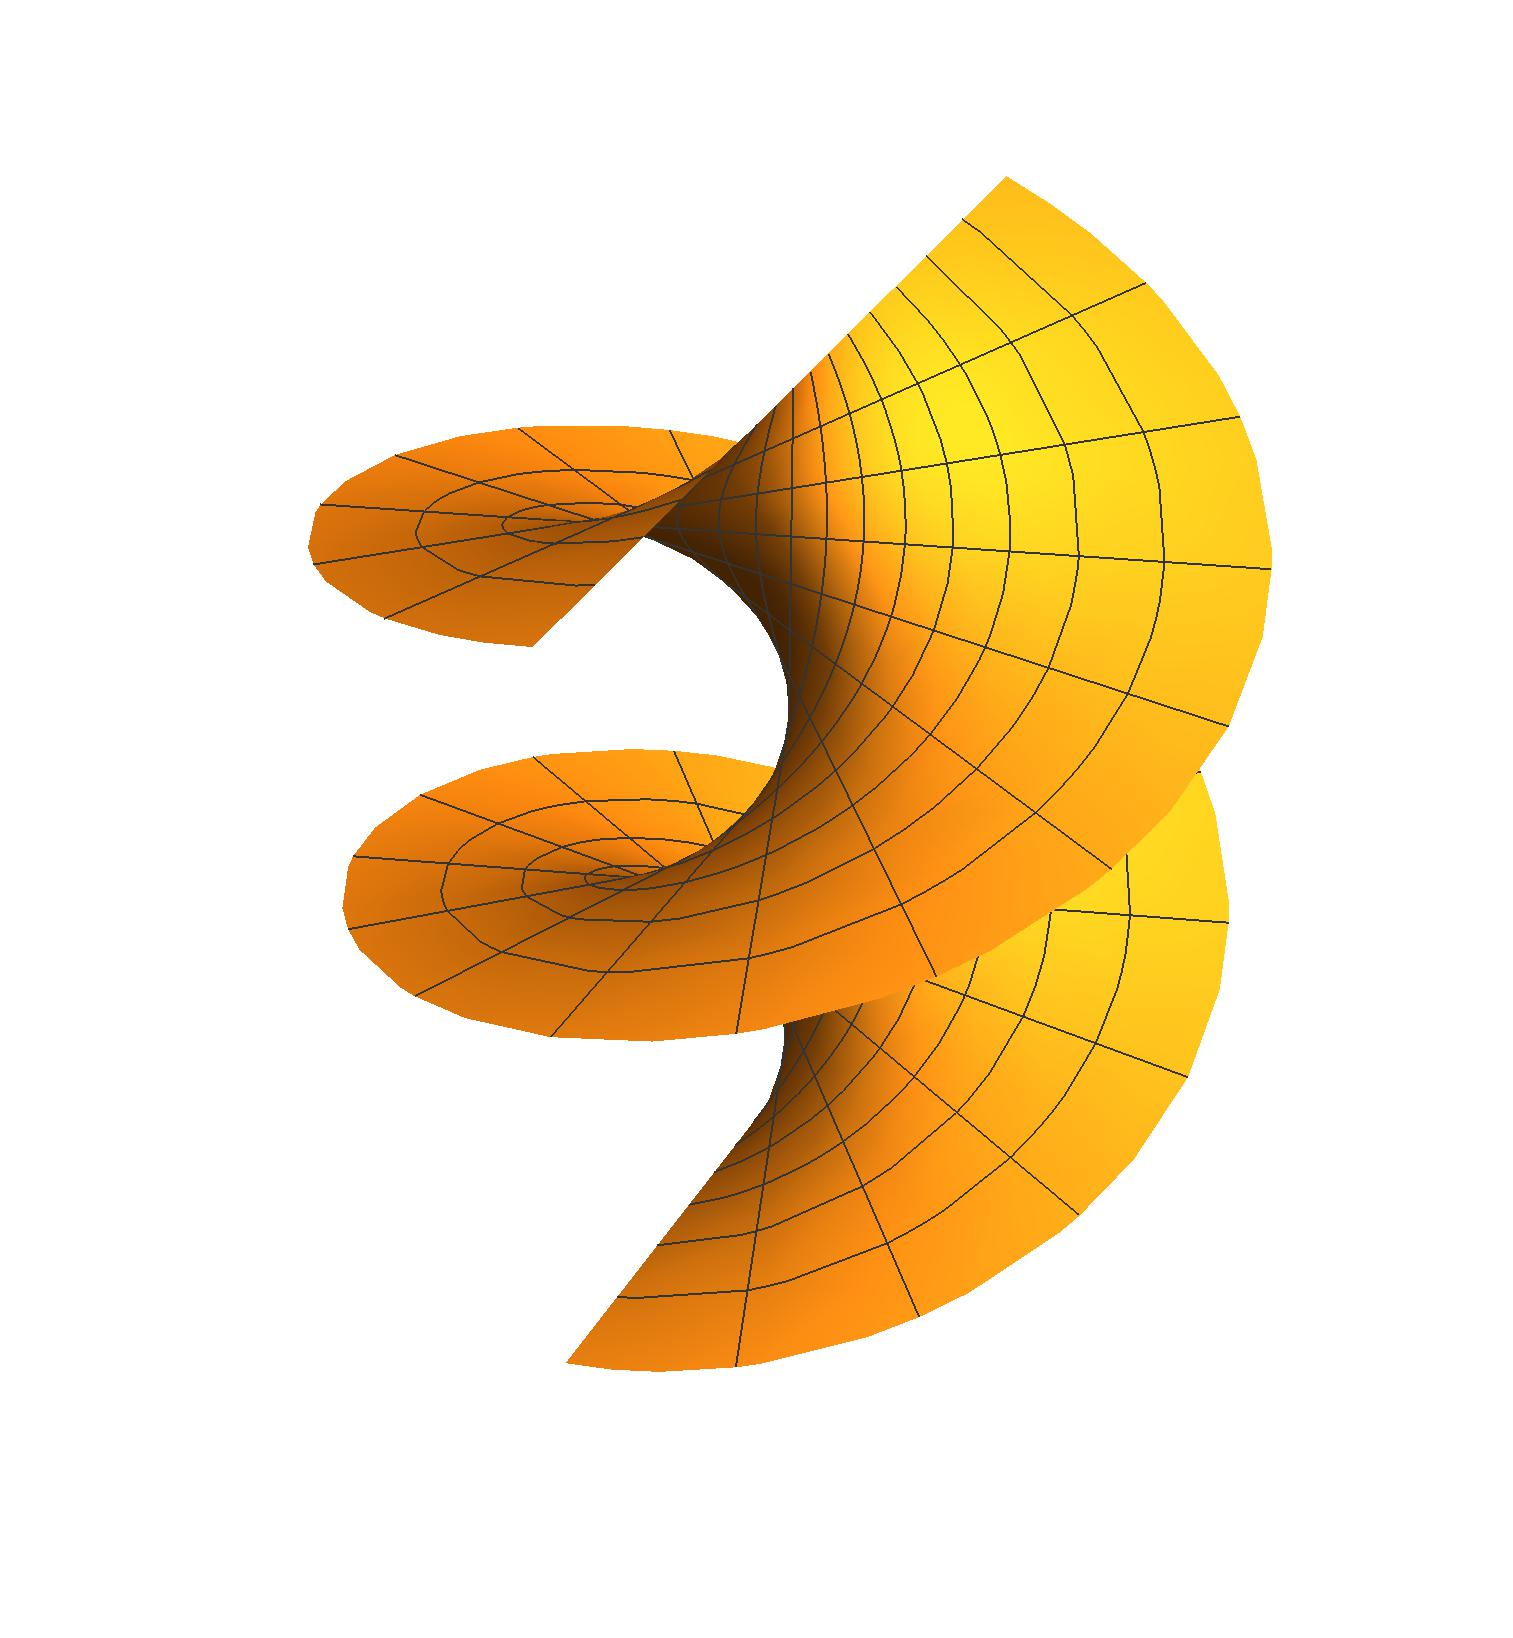
\includegraphics[scale=0.4]{helikoid.jpg}
\end{center}

\end{frame}

%%%%%%%%%%%%%%%%%%%%%%%%%%%%%%%%%%%%%%%%%%%

\begin{frame}
\frametitle{Primeri minimalnih ploskev -- Scherkovi ploskvi}

\begin{align*}
e^{z} \cos y &= \cos x & \sin z &= \sinh x \sinh y
\end{align*}

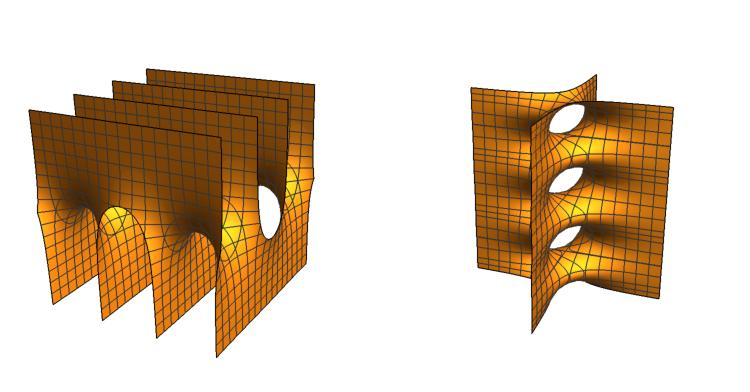
\includegraphics[scale=0.8]{scherk.jpg}

\end{frame}

%%%%%%%%%%%%%%%%%%%%%%%%%%%%%%%%%%%%%%%%%%%

\end{document}